% Copyright 2006 by Till Tantau
%
% This file may be distributed and/or modified
%
% 1. under the LaTeX Project Public License and/or
% 2. under the GNU Free Documentation License.
%
% See the file doc/generic/pgf/licenses/LICENSE for more details.


\section{Coordinate, Canvas, and Nonlinear Transformations}

\subsection{Overview}

\pgfname\ offers different ways of scaling, shifting, and rotating (these
operations are generally known as \emph{transformations}) graphics: You can
apply \emph{coordinate transformations} to all coordinates, you can apply
\emph{canvas transformations} to the canvas on which you draw, and you can
apply \emph{additional nonlinear transformations}. (The names ``coordinate''
and ``canvas'' transformations are not standard, I introduce them only for the
purposes of this manual.)

The differences are the following:
%
\begin{itemize}
    \item As the name ``coordinate transformation'' suggests, coordinate
        transformations apply only to coordinates. For example, when you
        specify a coordinate like |\pgfpoint{1cm}{2cm}| and you wish to ``use''
        this coordinate -- for example as an argument to a |\pgfpathmoveto|
        command -- then the coordinate transformation matrix is applied to the
        coordinate, resulting in a new coordinate. Continuing the example, if
        the current coordinate transformation is ``scale by a factor of two'',
        the coordinate |\pgfpoint{1cm}{2cm}| actually designates the point
        $(2\mathrm{cm},4\mathrm{cm})$.

        Note that coordinate transformations apply \emph{only} to coordinates.
        They do not apply to, say, line width or shadings or text.
    \item The effect of a ``canvas transformation'' like ``scale by a factor of
        two'' can be imagined as follows: You first draw your picture on a
        ``rubber canvas'' normally. Then, once you are done, the whole canvas
        is transformed, in this case stretched by a factor of two. In the
        resulting image \emph{everything} will be larger: Text, lines,
        coordinates, and shadings.
    \item Nonlinear transformations are a special form of coordinate
        transformations that are, as the name suggests, not linear. The support
        for nonlinear transformations is quite different from the support for
        linear coordinate transformations, the main reason being speed: While
        linear coordinate transformations can be applied very quickly
        (\pgfname\ does so almost constantly), nonlinear transformations are
        much harder to apply and also to use. For this reason, nonlinear
        transformations are implemented in a special module
        |nonlineartransformations| that has to be loaded explicitly. By
        default, they are not available.
\end{itemize}

In many cases, it is preferable that you use coordinate transformations and not
canvas transformations. When canvas transformations are used, \pgfname\ looses
track of the coordinates of nodes and shapes. Also, canvas transformations
often cause undesirable effects like changing text size. For these reasons,
\pgfname\ makes it easy to setup the coordinate transformation, but a bit
harder to change the canvas transformation. Because of the speed penalties
caused by nonlinear transformations, they are even harder to set up.


\subsection{Coordinate Transformations}
\label{section-linear-coordinate-transformations}

\subsubsection{How PGF Keeps Track of the Coordinate Transformation Matrix}
\label{section-transform-cm}

\pgfname\ has an internal coordinate transformation matrix. This matrix is
applied to coordinates ``in certain situations''. This means that the matrix is
not always applied to every coordinate ``no matter what''. Rather, \pgfname\
tries to be reasonably smart at when and how this matrix should be applied. The
most prominent examples are the path construction commands, which apply the
coordinate transformation matrix to their inputs.

The coordinate transformation matrix consists of four numbers $a$, $b$, $c$,
and $d$, and two dimensions $s$ and $t$. When the coordinate transformation
matrix is applied to a coordinate $(x,y)$, the new coordinate
$(ax+cy+s,bx+dy+t)$ results. For more details on how transformation matrices
work in general, please see, for example, the \textsc{pdf} or PostScript
reference or a textbook on computer graphics.

The coordinate transformation matrix is equal to the identity matrix at the
beginning. More precisely, $a=1$, $b=0$, $c=0$, $d=1$, $s=0\mathrm{pt}$, and
$t=0\mathrm{pt}$.

The different coordinate transformation commands will modify the matrix by
concatenating it with another transformation matrix. This way the effect of
applying several transformation commands will \emph{accumulate}.

The coordinate transformation matrix is local to the current \TeX\ group
(unlike the canvas transformation matrix, which is local to the current
|{pgfscope}|). Thus, the effect of adding a coordinate transformation to the
coordinate transformation matrix will last only till the end of the current
\TeX\ group.


\subsubsection{Commands for Relative Coordinate Transformations}

The following commands add a basic coordinate transformation to the current
coordinate transformation matrix. For all commands, the transformation is
applied \emph{in addition} to any previous coordinate transformations.

\begin{command}{\pgftransformshift\marg{point}}
    Shifts coordinates by \meta{point}.
    %
\begin{codeexample}[]
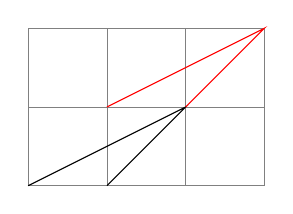
\begin{tikzpicture}
  \draw[help lines] (0,0) grid (3,2);
  \draw      (0,0) -- (2,1) -- (1,0);
  \pgftransformshift{\pgfpoint{1cm}{1cm}}
  \draw[red] (0,0) -- (2,1) -- (1,0);
\end{tikzpicture}
\end{codeexample}
    %
\end{command}

\begin{command}{\pgftransformxshift\marg{dimensions}}
    Shifts coordinates by \meta{dimension} along the $x$-axis.
    %
\begin{codeexample}[]
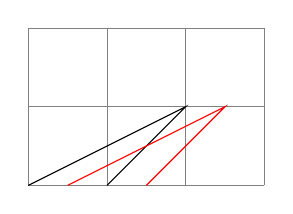
\begin{tikzpicture}
  \draw[help lines] (0,0) grid (3,2);
  \draw      (0,0) -- (2,1) -- (1,0);
  \pgftransformxshift{.5cm}
  \draw[red] (0,0) -- (2,1) -- (1,0);
\end{tikzpicture}
\end{codeexample}
    %
\end{command}

\begin{command}{\pgftransformyshift\marg{dimensions}}
    Like |\pgftransformxshift|, only for the $y$-axis.
\end{command}

\begin{command}{\pgftransformscale\marg{factor}}
    Scales coordinates by \meta{factor}.
    %
\begin{codeexample}[]
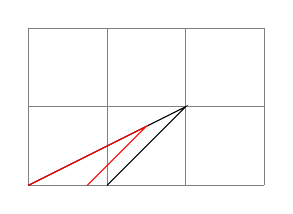
\begin{tikzpicture}
  \draw[help lines] (0,0) grid (3,2);
  \draw      (0,0) -- (2,1) -- (1,0);
  \pgftransformscale{.75}
  \draw[red] (0,0) -- (2,1) -- (1,0);
\end{tikzpicture}
\end{codeexample}
    %
\end{command}

\begin{command}{\pgftransformxscale\marg{factor}}
    Scales coordinates by \meta{factor} in the $x$-direction.
    %
\begin{codeexample}[]
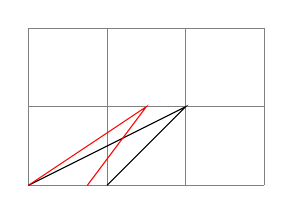
\begin{tikzpicture}
  \draw[help lines] (0,0) grid (3,2);
  \draw      (0,0) -- (2,1) -- (1,0);
  \pgftransformxscale{.75}
  \draw[red] (0,0) -- (2,1) -- (1,0);
\end{tikzpicture}
\end{codeexample}
    %
\end{command}

\begin{command}{\pgftransformyscale\marg{factor}}
    Like |\pgftransformxscale|, only for the $y$-axis.
\end{command}

\begin{command}{\pgftransformxslant\marg{factor}}
    Slants coordinates by \meta{factor} in the $x$-direction. Here, a factor of
    |1| means $45^\circ$.
    %
\begin{codeexample}[]
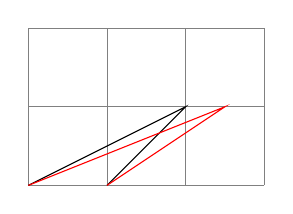
\begin{tikzpicture}
  \draw[help lines] (0,0) grid (3,2);
  \draw      (0,0) -- (2,1) -- (1,0);
  \pgftransformxslant{.5}
  \draw[red] (0,0) -- (2,1) -- (1,0);
\end{tikzpicture}
\end{codeexample}
    %
\end{command}

\begin{command}{\pgftransformyslant\marg{factor}}
    Slants coordinates by \meta{factor} in the $y$-direction.
    %
\begin{codeexample}[]
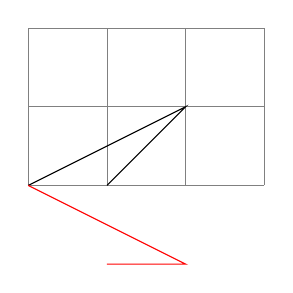
\begin{tikzpicture}
  \draw[help lines] (0,0) grid (3,2);
  \draw      (0,0) -- (2,1) -- (1,0);
  \pgftransformyslant{-1}
  \draw[red] (0,0) -- (2,1) -- (1,0);
\end{tikzpicture}
\end{codeexample}
    %
\end{command}


\begin{command}{\pgftransformrotate\marg{angles}}
    Rotates coordinates counterclockwise by \meta{angles} given in degrees.
    %
\begin{codeexample}[]
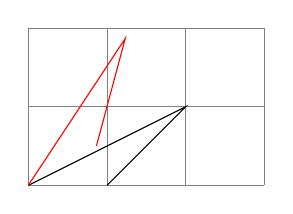
\begin{tikzpicture}
  \draw[help lines] (0,0) grid (3,2);
  \draw      (0,0) -- (2,1) -- (1,0);
  \pgftransformrotate{30}
  \draw[red] (0,0) -- (2,1) -- (1,0);
\end{tikzpicture}
\end{codeexample}
    %
\end{command}

\begin{command}{\pgftransformtriangle\marg{a}\marg{b}\marg{c}}
    This command transforms the coordinate system in such a way that the
    triangle given by the points \meta{a}, \meta{b} and \meta{c} lies at the
    coordinates $(0,0)$, $(1\mathrm{pt},0\mathrm{pt})$ and
    $(0\mathrm{pt},1\mathrm{pt})$.
    %
\begin{codeexample}[]
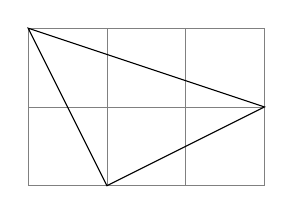
\begin{tikzpicture}
  \draw[help lines] (0,0) grid (3,2);
  \pgftransformtriangle
  {\pgfpoint{1cm}{0cm}}
  {\pgfpoint{0cm}{2cm}}
  {\pgfpoint{3cm}{1cm}}

  \draw (0,0) -- (1pt,0pt) -- (0pt,1pt) -- cycle;
\end{tikzpicture}
\end{codeexample}
    %
\end{command}

\begin{command}{\pgftransformcm\marg{a}\marg{b}\marg{c}\marg{d}\marg{point}}
    Applies the transformation matrix given by $a$, $b$, $c$, and $d$ and the
    shift \meta{point} to coordinates (in addition to any previous
    transformations already in force).
    %
\begin{codeexample}[]
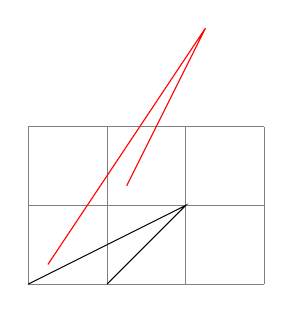
\begin{tikzpicture}
  \draw[help lines] (0,0) grid (3,2);
  \draw      (0,0) -- (2,1) -- (1,0);
  \pgftransformcm{1}{1}{0}{1}{\pgfpoint{.25cm}{.25cm}}
  \draw[red] (0,0) -- (2,1) -- (1,0);
\end{tikzpicture}
\end{codeexample}
    %
\end{command}

\begin{command}{\pgftransformarrow\marg{start}\marg{end}}
    Shifts coordinates to the end of the line going from \meta{start} to
    \meta{end} with the correct rotation.
    %
\begin{codeexample}[]
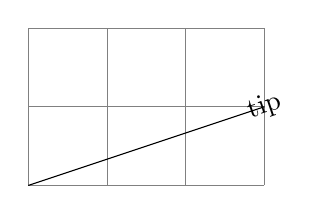
\begin{tikzpicture}
  \draw[help lines] (0,0) grid (3,2);
  \draw      (0,0) -- (3,1);
  \pgftransformarrow{\pgfpointorigin}{\pgfpoint{3cm}{1cm}}
  \pgftext{tip}
\end{tikzpicture}
\end{codeexample}
    %
\end{command}

\begin{command}{\pgftransformlineattime\marg{time}\marg{start}\marg{end}}
    Shifts coordinates by a specific point on a line at a specific time. The
    point by which the coordinate is shifted is calculated by calling
    |\pgfpointlineattime|, see Section~\ref{section-pointsattime}.

    In addition to shifting the coordinate, a rotation \emph{may} also be
    applied. Whether this is the case depends on whether the \TeX\ if
    |\ifpgfslopedattime| is set to true or not.
    %
\begin{codeexample}[]
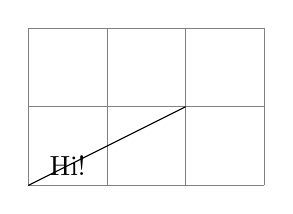
\begin{tikzpicture}
  \draw[help lines] (0,0) grid (3,2);
  \draw      (0,0) -- (2,1);
  \pgftransformlineattime{.25}{\pgfpointorigin}{\pgfpoint{2cm}{1cm}}
  \pgftext{Hi!}
\end{tikzpicture}
\end{codeexample}
    %
\begin{codeexample}[]
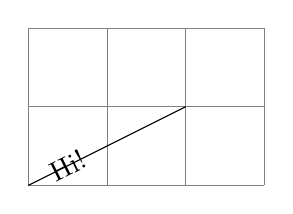
\begin{tikzpicture}
  \draw[help lines] (0,0) grid (3,2);
  \draw      (0,0) -- (2,1);
  \pgfslopedattimetrue
  \pgftransformlineattime{.25}{\pgfpointorigin}{\pgfpoint{2cm}{1cm}}
  \pgftext{Hi!}
\end{tikzpicture}
\end{codeexample}
    %
    If |\ifpgfslopedattime| is true, another \TeX\ |\if| is important:
    |\ifpgfallowupsidedowattime|. If this is false, \pgfname\ will ensure that
    the rotation is done in such a way that text is never ``upside down''.

    There is another \TeX\ |\if| that influences this command. If you set
    |\ifpgfresetnontranslationattime| to true, then, between shifting the
    coordinate and (possibly) rotating/sloping the coordinate, the command
    |\pgftransformresetnontranslations| is called. See the description of this
    command for details.
    %
\begin{codeexample}[]
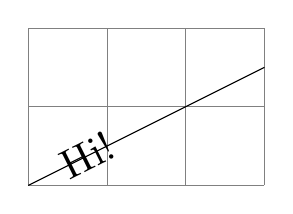
\begin{tikzpicture}
  \draw[help lines] (0,0) grid (3,2);
  \pgftransformscale{1.5}
  \draw      (0,0) -- (2,1);
  \pgfslopedattimetrue
  \pgfresetnontranslationattimefalse
  \pgftransformlineattime{.25}{\pgfpointorigin}{\pgfpoint{2cm}{1cm}}
  \pgftext{Hi!}
\end{tikzpicture}
\end{codeexample}
    %
\begin{codeexample}[]
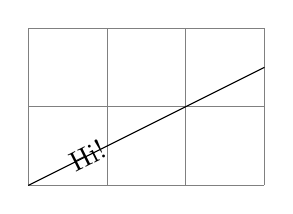
\begin{tikzpicture}
  \draw[help lines] (0,0) grid (3,2);
  \pgftransformscale{1.5}
  \draw      (0,0) -- (2,1);
  \pgfslopedattimetrue
  \pgfresetnontranslationattimetrue
  \pgftransformlineattime{.25}{\pgfpointorigin}{\pgfpoint{2cm}{1cm}}
  \pgftext{Hi!}
\end{tikzpicture}
\end{codeexample}
    %
\end{command}

\begin{command}{\pgftransformcurveattime\marg{time}\marg{start}\marg{first support}\marg{second support}\marg{end}}
    Shifts coordinates by a specific point on a curve at a specific time, see
    Section~\ref{section-pointsattime} once more.

    As for the line-at-time transformation command, |\ifpgfslopedattime|
    decides whether an additional rotation should be applied. Again, the value
    of |\ifpgfallowupsidedowattime| is also considered.
    %
\begin{codeexample}[]
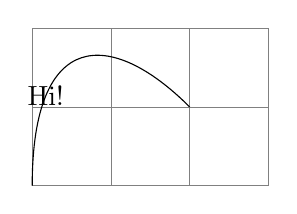
\begin{tikzpicture}
  \draw[help lines] (0,0) grid (3,2);
  \draw      (0,0) .. controls (0,2) and (1,2) .. (2,1);
  \pgftransformcurveattime{.25}{\pgfpointorigin}
    {\pgfpoint{0cm}{2cm}}{\pgfpoint{1cm}{2cm}}{\pgfpoint{2cm}{1cm}}
  \pgftext{Hi!}
\end{tikzpicture}
\end{codeexample}
    %
\begin{codeexample}[]
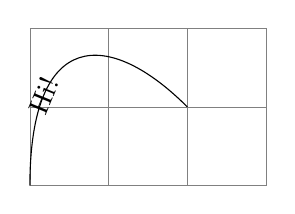
\begin{tikzpicture}
  \draw[help lines] (0,0) grid (3,2);
  \draw      (0,0) .. controls (0,2) and (1,2) .. (2,1);
  \pgfslopedattimetrue
  \pgftransformcurveattime{.25}{\pgfpointorigin}
    {\pgfpoint{0cm}{2cm}}{\pgfpoint{1cm}{2cm}}{\pgfpoint{2cm}{1cm}}
  \pgftext{Hi!}
\end{tikzpicture}
\end{codeexample}
    %
    The value of |\ifpgfresetnontranslationsattime| is also taken into account.
\end{command}

\begin{command}{\pgftransformarcaxesattime\marg{time
      $t$}\marg{center}\marg{0-degree axis}\marg{90-degree
      axis}\marg{start angle}\marg{end angle}%
}
    Shifts coordinates by a specific point on an arc at a specific time, see
    Section~\ref{section-pointsattime} once more.

    As for the previous commands, |\ifpgfslopedattime| decides whether an
    additional rotation should be applied and |\ifpgfallowupsidedowattime| is
    also considered.
    %
\begin{codeexample}[]
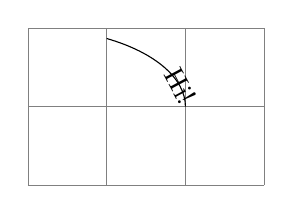
\begin{tikzpicture}
  \draw[help lines] (0,0) grid (3,2);
  \pgfpathmoveto{\pgfpoint{2cm}{1cm}}
  \pgfpatharcaxes{0}{60}{\pgfpoint{2cm}{0cm}}{\pgfpoint{0cm}{1cm}}
  \pgfusepath{stroke}
  \pgfslopedattimetrue
  \pgftransformarcaxesattime{.25}
    {\pgfpoint{0cm}{1cm}}
    {\pgfpoint{2cm}{0cm}}{\pgfpoint{0cm}{1cm}}
    {0}{60}
  \pgftext{Hi!}
\end{tikzpicture}
\end{codeexample}
    %
    The value of |\ifpgfresetnontranslationsattime| is also taken into account.
\end{command}

{
    \let\ifpgfslopedattime=\relax
    \begin{textoken}{\ifpgfslopedattime}
        Decides whether the ``at time'' transformation commands also rotate
        coordinates or not.
    \end{textoken}
}
{
    \let\ifpgfallowupsidedowattime=\relax
    \begin{textoken}{\ifpgfallowupsidedowattime}
        Decides whether the ``at time'' transformation commands should allow
        the rotation be done in such a way that ``upside-down text'' can
        result.
    \end{textoken}
}
{
    \let\ifpgfresetnontranslationsattime=\relax
    \begin{textoken}{\ifpgfresetnontranslationsattime}
        Decides whether the ``at time'' transformation commands should reset
        the non-translations between shifting and rotating.
    \end{textoken}
}


\subsubsection{Commands for Absolute Coordinate Transformations}

The coordinate transformation commands introduced up to now are always applied
in addition to any previous transformations. In contrast, the commands
presented in the following can be used to change the transformation matrix ``in
absolute terms''. Note that this is, in general, dangerous and will often
produce unexpected effects. You should use these commands only if you really
know what you are doing.

\begin{command}{\pgftransformreset}
    Resets the coordinate transformation matrix to the identity matrix. Thus,
    once this command is given no transformations are applied till the end of
    the scope.
    %
\begin{codeexample}[]
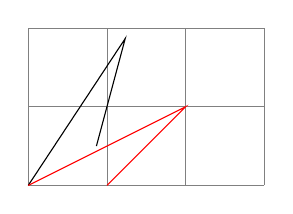
\begin{tikzpicture}
  \draw[help lines] (0,0) grid (3,2);
  \pgftransformrotate{30}
  \draw      (0,0) -- (2,1) -- (1,0);
  \pgftransformreset
  \draw[red] (0,0) -- (2,1) -- (1,0);
\end{tikzpicture}
\end{codeexample}
    %
\end{command}

\begin{command}{\pgftransformresetnontranslations}
    This command sets the $a$, $b$, $c$, and $d$ part of the coordinate
    transformation matrix to $a=1$, $b=0$, $c=0$, and $d=1$. However, the
    current shifting of the matrix is not modified.

    The effect of this command is that any rotation/scaling/slanting is undone
    in the current \TeX\ group, but the origin is not ``moved back''.

    This command is mostly useful directly before a |\pgftext| command to
    ensure that the text is not scaled or rotated.
    %
\begin{codeexample}[]
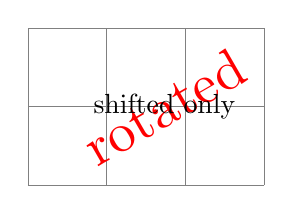
\begin{tikzpicture}
  \draw[help lines] (0,0) grid (3,2);
  \pgftransformscale{2}
  \pgftransformrotate{30}
  \pgftransformxshift{1cm}
  {\color{red}\pgftext{rotated}}
  \pgftransformresetnontranslations
  \pgftext{shifted only}
\end{tikzpicture}
\end{codeexample}
    %
\end{command}

\begin{command}{\pgftransforminvert}
    Replaces the coordinate transformation matrix by a coordinate
    transformation matrix that ``exactly undoes the original transformation''.
    For example, if the original transformation was ``scale by 2 and then shift
    right by 1cm'' the new one is ``shift left by 1cm and then scale by
    $1/2$''.

    This command will produce an error if the determinant of the matrix is too
    small, that is, if the matrix is near-singular.
    %
\begin{codeexample}[]
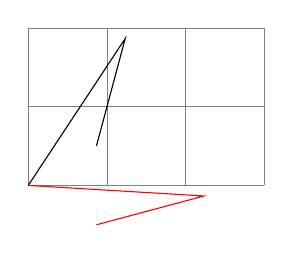
\begin{tikzpicture}
  \draw[help lines] (0,0) grid (3,2);
  \pgftransformrotate{30}
  \draw      (0,0) -- (2,1) -- (1,0);
  \pgftransforminvert
  \draw[red] (0,0) -- (2,1) -- (1,0);
\end{tikzpicture}
\end{codeexample}
    %
\end{command}


\subsubsection{Saving and Restoring the Coordinate Transformation Matrix}

There are two commands for saving and restoring coordinate transformation
matrices.

\begin{command}{\pgfgettransform\marg{macro}}
    This command will (locally) define \meta{macro} to a representation of the
    current coordinate transformation matrix. This matrix can later on be
    reinstalled using |\pgfsettransform|.
\end{command}

\begin{command}{\pgfsettransform\marg{macro}}
    Reinstalls a coordinate transformation matrix that was previously saved
    using |\pgfgettransform|.
\end{command}

\begin{command}{\pgfgettransformentries\marg{macro for a}\marg{macro
      for b}\marg{macro for c}\marg{macro for d}\marg{macro for shift
      x}\marg{macro for shift y}%
}
    This command is similar to |\pgfgettransform| except that it stores the
    current coordinate transformation matrix in a set of six macros.

    The matrix can later on be reinstalled using |\pgfsettransformentries|.
    Furthermore, all these macros (or just a few of them) can be used as
    arguments for |\pgftransformcm|.
\end{command}

\begin{command}{\pgfsettransformentries\marg{a}\marg{b}\marg{c}\marg{d}\marg{shiftx}\marg{shifty}}
    Reinstalls a coordinate transformation matrix that was previously saved
    using the storage command |\pgfgettransformentries|. This command can also
    be used to replace any previously existing coordinate transformation matrix
    (it is thus equivalent to |\pgftransformreset| followed by
    |\pgftransformcm|).
\end{command}


\subsubsection{Computing Adjustments for Coordinate Transformations}
\label{section-adjustment-transformations}

\begin{command}{\pgftransformationadjustments}
    This command computes ``adjustments'' for the current transformation matrix
    so that even when you install a transformation matrix that scales
    everything by a certain factor, you can still draw something of ``an
    absolute size''. Suppose for instance that you install a transformation
    matrix that scales everything by a factor of 4 and you now wish to draw a
    horizontal line of length 1cm. Then, if you do not reset the transformation
    matrix, you can draw a line of logical length 2.5mm, which will then get
    scaled to a line of 1cm. Things get more difficult in case you scale things
    only, say, vertically. In this case, the adjustment necessary for
    horizontal lines is different from the one needed for vertical lines.

    This function computes two scaling factors, one for horizontal lines
    and one for vertical lines, and stores them in the following macros:
    %
    \begin{command}{\pgfhorizontaltransformationadjustment}
        When you scale the length of a horizontal line by this factor in the
        current transformation, you compensate for the scaling. Formally, it is
        $1/\|\mathit{transform}(1,0)\|_2$, where $\mathit{transform}$ applies
        the current transformations matrix to the given number.
        %
\begin{codeexample}[]
\begin{tikzpicture}
  \draw [help lines] (0,0) grid (2,2);
  \begin{scope}[xscale=2,thick]
    \draw [red] (1,1) -- ++(1,0);

    \pgftransformationadjustments
    \draw [blue] (1,0) -- ++(\pgfhorizontaltransformationadjustment,0);
  \end{scope}
\end{tikzpicture}
\end{codeexample}
        %
\begin{codeexample}[]
\begin{tikzpicture}
  \draw [help lines] (0,0) grid (2,2);
  \begin{scope}[xscale=2,thick,rotate=90]
    \draw [red] (1,1) -- ++(1,0);

    \pgftransformationadjustments
    \draw [blue] (1,0) -- ++(\pgfhorizontaltransformationadjustment,0);
  \end{scope}
\end{tikzpicture}
\end{codeexample}
    \end{command}
    %
    \begin{command}{\pgfverticaltransformationadjustment}
        $1/\|\mathit{transform}(0,1)\|_2$.
    \end{command}

    Note that the ``right'' way to draw a line of absolute length 1cm in a
    transformed coordinate system is to first compute the start point and to
    then reset the transformation matrix. The transformation adjustments
    computed here are important only in situations where you cannot do this,
    for instance when an |outer xsep| must be set.
\end{command}


\subsection{Canvas Transformations}

The canvas transformation matrix is not managed by \pgfname, but by the output
format like \pdf\ or PostScript. All that \pgfname\ does is to call appropriate
low-level |\pgfsys@| commands to change the canvas transformation matrix.

Unlike coordinate transformations, canvas transformations apply to
``everything'', including images, text, shadings, line thickness, and so on.
The idea is that a canvas transformation really stretches and deforms the
canvas after the graphic is finished.

Unlike coordinate transformations, canvas transformations are local to the
current |{pgfscope}|, not to the current \TeX\ group. This is due to the fact
that they are managed by the backend driver, not by \TeX\ or \pgfname.

Unlike the coordinate transformation matrix, it is not possible to ``reset''
the canvas transformation matrix. The only way to change it is to concatenate
it with another canvas transformation matrix or to end the current
|{pgfscope}|.

Unlike coordinate transformations, \pgfname\ does not ``keep track'' of canvas
transformations. In particular, it will not be able to correctly save the
coordinates of shapes or nodes when a canvas transformation is used.


\subsubsection{Applying General Canvas Transformations}

\pgfname\ does not offer many commands for modifying the canvas transformation
matrix. Instead, different commands allow you to concatenate the canvas
transformation matrix with a coordinate transformation matrix (and there are
numerous commands for specifying a coordinate transformation, see the previous
section).

\begin{command}{\pgflowlevelsynccm}
    This command concatenates the canvas transformation matrix with the current
    coordinate transformation matrix. Afterward, the coordinate transformation
    matrix is reset.

    The effect of this command is to ``synchronize'' the coordinate
    transformation matrix and the canvas transformation matrix. All
    transformations that were previously applied by the coordinate
    transformations matrix are now applied by the canvas transformation matrix.
    %
\begin{codeexample}[]
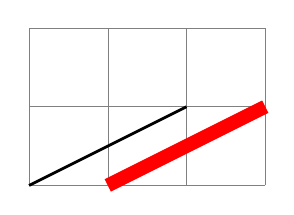
\begin{tikzpicture}
  \draw[help lines] (0,0) grid (3,2);
  \pgfsetlinewidth{1pt}
  \pgftransformscale{5}
  \draw      (0,0) -- (0.4,.2);
  \pgftransformxshift{0.2cm}
  \pgflowlevelsynccm
  \draw[red] (0,0) -- (0.4,.2);
\end{tikzpicture}
\end{codeexample}
    %
\end{command}

\begin{command}{\pgflowlevel\marg{transformation code}}
    This command concatenates the canvas transformation matrix with the
    coordinate transformation specified by \meta{transformation code}.
    %
\begin{codeexample}[]
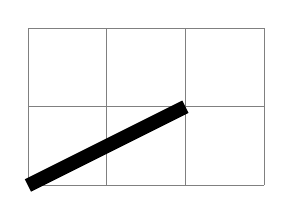
\begin{tikzpicture}
  \draw[help lines] (0,0) grid (3,2);
  \pgfsetlinewidth{1pt}
  \pgflowlevel{\pgftransformscale{5}}
  \draw      (0,0) -- (0.4,.2);
\end{tikzpicture}
\end{codeexample}
    %
\end{command}

\begin{command}{\pgflowlevelobj\marg{transformation code}\marg{code}}
    This command creates a local |{pgfscope}|. Inside this scope,
    |\pgflowlevel| is first called with the argument \meta{transformation
    code}, then the \meta{code} is inserted.
    %
\begin{codeexample}[]
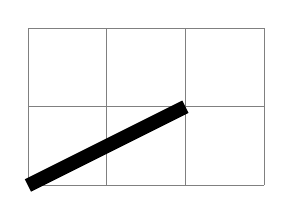
\begin{tikzpicture}
  \draw[help lines] (0,0) grid (3,2);
  \pgfsetlinewidth{1pt}
  \pgflowlevelobj{\pgftransformscale{5}}    {\draw (0,0) -- (0.4,.2);}
  \pgflowlevelobj{\pgftransformxshift{-1cm}}{\draw (0,0) -- (0.4,.2);}
\end{tikzpicture}
\end{codeexample}
    %
\end{command}

\begin{environment}{{pgflowlevelscope}\marg{transformation code}}
    This environment first surrounds the \meta{environment contents} by a
    |{pgfscope}|. Then it calls |\pgflowlevel| with the argument
    \meta{transformation code}.
    %
\begin{codeexample}[]
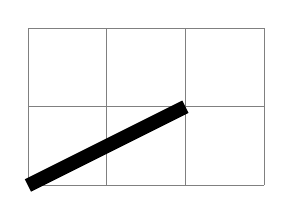
\begin{tikzpicture}
  \draw[help lines] (0,0) grid (3,2);
  \pgfsetlinewidth{1pt}
  \begin{pgflowlevelscope}{\pgftransformscale{5}}
    \draw (0,0) -- (0.4,.2);
  \end{pgflowlevelscope}
  \begin{pgflowlevelscope}{\pgftransformxshift{-1cm}}
    \draw (0,0) -- (0.4,.2);
  \end{pgflowlevelscope}
\end{tikzpicture}
\end{codeexample}
    %
\end{environment}

\begin{plainenvironment}{{pgflowlevelscope}\marg{transformation code}}
    Plain \TeX\ version of the environment.
\end{plainenvironment}

\begin{contextenvironment}{{pgflowlevelscope}\marg{transformation code}}
    Con\TeX t version of the environment.
\end{contextenvironment}


\subsubsection{Establishing View Boxes}
\label{section-base-view}

A \emph{view box} is like a ``window'' through which you see a graphic. To
establish a view box, you specify a rectangle -- which is the window -- and
another rectangle surrounding the to-be-viewed graphic. The graphic will then
be rescaled and shifted in such a way that the to-be-viewed rectangle matches
the view box's rectangle as well as possible. Note that establishing a view box
does, indeed, cause a canvas transformation to be installed.

View boxes are only seldom needed in normal graphics. Their main application is
with animations since you can \emph{animate} the to-be-viewed rectangle. This
makes it easy to create animations in which you zoom in, zoom out, and pan a
graphic.

\begin{environment}{{pgfviewboxscope}\marg{$ll_1$}\marg{$ur_1$}\marg{$ll_2$}\marg{$ur_2$}\marg{meet or slice}}
    Inside the viewbox scope, the source rectangle (with the two \pgfname\
    points $ll_1$ and $ur_1$ as corners) will be translated and scaled so that
    it becomes centered on the target rectangle (with the corners $ll_2$ and
    $ur_2$) and will, for |meet| as last parameter, be as large as possible so
    that it fits inside the target and, for |slice|, be as small as possible so
    that it encompasses the target.
    %
\begin{codeexample}[]
\tikz {
  \draw [red, very thick] (0,0) rectangle (20mm,20mm);
  \begin{pgfviewboxscope}
    {\pgfpoint{5mm}{5mm}}{\pgfpoint{25mm}{15mm}} % Source
    {\pgfpoint{0mm}{0mm}}{\pgfpoint{20mm}{20mm}} % Target
    {meet}
    \draw [blue, very thick] (5mm,5mm) rectangle (25mm,15mm);
    \draw [thick] (1,1) circle [radius=8mm] node {Hi};
  \end{pgfviewboxscope} }
\end{codeexample}
    %
\begin{codeexample}[]
\tikz {
  \draw [red, very thick] (0,0) rectangle (20mm,20mm);
  \begin{pgfviewboxscope}
    {\pgfpoint{5mm}{5mm}}{\pgfpoint{25mm}{15mm}} % Source
    {\pgfpoint{0mm}{0mm}}{\pgfpoint{20mm}{20mm}} % Target
    {slice}
    \draw [blue, very thick] (5mm,5mm) rectangle (25mm,15mm);
    \draw [thick] (1,1) circle [radius=8mm] node {Hi};
  \end{pgfviewboxscope} }
\end{codeexample}
    %
\end{environment}

\begin{plainenvironment}{{pgfviewboxscope}\marg{$ll_1$}\marg{$ur_1$}\marg{$ll_2$}\marg{$ur_2$}\marg{meet or slice}}
    Plain \TeX\ version of the environment.
\end{plainenvironment}

\begin{contextenvironment}{{pgfviewboxscope}\marg{$ll_1$}\marg{$ur_1$}\marg{$ll_2$}\marg{$ur_2$}\marg{meet or slice}}
    Con\TeX t version of the environment.
\end{contextenvironment}


\subsection{Nonlinear Transformations}
\label{section-nonlinear-transformations}

In order to use nonlinear transformations, you first have to load the following
\pgfname\ module:

\begin{pgfmodule}{nonlineartransformations}
    Loads the necessary functionality for nonlinear transformations.
\end{pgfmodule}


\subsubsection{Introduction}

The difference between the coordinate transformations introduced in
Section~\ref{section-linear-coordinate-transformations} above to nonlinear
transformations is, of course, that the transformations can be nonlinear. An
example of a nonlinear transformation is the transformation underlying polar
coordinates: A polar coordinate $(r,d)$ gets transformed to the canvas position
$(d\cos r,d\sin r)$, which is clearly not a linear transformation.

Nonlinear transformations work somewhat like the normal linear coordinate
transformations in the sense that they apply to coordinate and thereby to the
construction of paths, but not to things like text or line width or shadings.
(Indeed, it is not possible to apply nonlinear transformations to, say, text.)

This means that there is a fundamental difference between, on the one hand,
calling a function like |\pgfpointpolar| or specifying a coordinate as |(45:2)|
in \tikzname\ and, on the other hand, installing the nonlinear transformation
``polar coordinates'' using the command |\pgftransformnonlinear|: In a
coordinate like |(45:2)| the user explicitly says ``please evaluate this one
coordinate in polar coordinate and then continue in the normal coordinate
system with the result''. Otherwise nothing changes and a line between two
points specified in this way is still a straight line.

Things are quite different when we install a polar \emph{transformation} using
|\pgftransformnonlinear|. Now, even a seemingly low-level Cartesian coordinate
|\pgfqpoint{1pt}{1pt}| will get transformed. Even more drastically, what is
specified as a straight line like
%
\begin{codeexample}[code only]
\draw (0,1) -- (1,1);
\end{codeexample}
%
can become curved since \emph{everything} gets transformed.


\subsubsection{Installing Nonlinear Transformation}

\begin{codeexample}[setup code,hidden]
\makeatletter
\def\polartransformation{
  % \pgf@x will contain the radius
  % \pgf@y will contain the distance
  \pgfmathsincos@{\pgf@sys@tonumber\pgf@x}%
  % pgfmathresultx is now the cosine of radius and
  % pgfmathresulty is the sine of radius
  \pgf@x=\pgfmathresultx\pgf@y%
  \pgf@y=\pgfmathresulty\pgf@y%
}
\makeatother
\end{codeexample}

\begin{command}{\pgftransformnonlinear\marg{transformation code}}
    This command adds the \meta{transformation code} to the list of non-linear
    transformations currently in force. Thus, similar to linear coordinate
    transformations, each additional call to this function adds another
    transformation to the current \TeX\ scope and the effect ends at the end of
    the current scope. In practice, however, you typically will not have more
    than one active nonlinear transformation.

    The job of the \meta{transformation code} is to map a point~$p$ given in
    the registers |\pgf@x| and |\pgf@y| to a new coordinate~$f(p)$, which
    should be returned in |\pgf@x| and |\pgf@y| as well. As an example, suppose
    we wish to install polar coordinates as the nonlinear transformation. For
    this, we need a bit of code:
    %
\begin{codeexample}[code only]
\def\polartransformation{%
  % \pgf@x will contain the radius
  % \pgf@y will contain the distance
  \pgfmathsincos@{\pgf@sys@tonumber\pgf@x}%
  % pgfmathresultx is now the cosine of radius and
  % pgfmathresulty is the sine of radius
  \pgf@x=\pgfmathresultx\pgf@y%
  \pgf@y=\pgfmathresulty\pgf@y%
}
\end{codeexample}
    %
    (In case you wonder why you cannot just call |\pgfpointpolar| at this
    point: You can, but this function internally uses |\pgf@x| and |\pgf@y| in
    complicated ways, so you would first have to safe them so some other
    registers. Also, the above is faster.)

    If we were to call this function again, we would get something funny like
    ``polar-polar coordinates'', so let's not do this. Let us instead have a
    look at the effect this call has: Once a nonlinear transformation is
    installed, all subsequent path constructions are affected by this
    transformation. In particular, a normal grid now becomes the typical
    ``polar grid''.
    %
\begin{codeexample}[preamble={\usepgfmodule{nonlineartransformations}}]
\begin{tikzpicture}
  \draw [help lines] (0,0) grid (3,2);
  % Start nonlinear transformation
  \pgftransformnonlinear{\polartransformation}% see above

  % Draw something with this transformation in force
  \draw (0pt,0mm) grid [xstep=10pt, ystep=5mm] (90pt, 20mm);
\end{tikzpicture}
\end{codeexample}
    %
\end{command}


\subsubsection{Applying Nonlinear Transformations to Points}

\begin{command}{\pgfpointtransformednonlinear\marg{point}}
    Works like |\pgfpointtransformed|, but also applies the current nonlinear
    transformation; that is, it first applies the current linear transformation
    and then the current nonlinear transformations. Note that, just like
    |\pgfpointtransformed|, you normally do not call this function directly
    since it is called internally by the path drawing commands.
\end{command}


\subsubsection{Applying Nonlinear Transformations to Paths}

When a nonlinear transformation is installed, the normal path construction
commands like |\pgfpathmoveto| get adjusted so that the ``honour'' the
nonlinear transformations currently in force. For |\pgfpathmoveto| this is
pretty simple: Instead of just applying the linear transformation matrix to the
point to which the path should ``jump'' next, we also apply the nonlinear
transformation. However, for a command like |\pgfpathlineto|, things are much
more difficult: A straight line will no longer be a straight line!

In order to make straight lines ``bend'', the following changes are in force
while a nonlinear transformation is installed:
%
\begin{enumerate}
    \item Whenever a straight line between two points $p$ and $q$ should be
        added to the path, either through |\pgfpathlineto| or through
        |\pgfpathclose|, we replace this straight line by a ``degenerated
        curve'' from $p$ to $q$ whose control points are at one third and two
        third of the distance between $p$ and $q$ on the line between $p$ and
        $q$. In this way, while nonlinear transformations are in force, we only
        need to transform curves.
    \item Next, suppose we wish to transform a curve from $p$ to $q$ with
        supports $s$ and $t$. For this, we simply apply the nonlinear
        transformation $f$ to all four points and draw a line with the results.
        Note that this mapping is actually not quite satisfactory for long
        lines that are strongly curved:
        %
\begin{codeexample}[preamble={\usepgfmodule{nonlineartransformations}}]
\begin{tikzpicture}
  \draw [help lines] (0,0) grid (3,2);
  {
    \pgftransformnonlinear{\polartransformation}
    % The curve with the controls computed by pgf: a nice quarter arc
    \draw [red] (0,20mm) -- (90pt,20mm);
  }
  % Here is the curve with controls just transformed:
  \draw (0:20mm) .. controls (30pt:20mm) and (60pt:20mm) .. (90pt:20mm);
\end{tikzpicture}
\end{codeexample}
        %
        As the example shows, the control points now lie on the arc; but in
        reality they should point along the tangents at the start and the end.
        This is exactly when \pgfname\ does through the computation described
        above.
    \item To overcome the effect of the control points being ``off'', it is
        necessary to split up longer curves into smaller parts, which are drawn
        individually to increase the accuracy. When such splitting occurs, can
        be configured using the following command:
        %
        \begin{command}{\pgfsettransformnonlinearflatness\marg{dimension} (initially 5pt)}
            Whenever in a to-be-drawn curve the $L^\infty$-distance (maximum of
            the distances in $x$- and $y$-directions) between the start of a
            curve and its first control point or between the first and second
            control points or between the second control point and the end is
            more than \meta{distance}, the curve gets split in the middle (more
            precisely, at time $t= 0.5$) and we draw the two parts individually
            (for them, splitting may occur again, if the curve is still too
            long).
            %
\begin{codeexample}[preamble={\usepgfmodule{nonlineartransformations}}]
\begin{tikzpicture}
  \draw [help lines] (0,0) grid (3,2);
  \draw[red] (0:20mm) arc [start angle=0, end angle=90, radius=2cm];
  {
    \pgftransformnonlinear{\polartransformation}
    \pgfsettransformnonlinearflatness{2pt} % very precise
    \draw (0,20mm) -- (90pt,20mm);
  }
\end{tikzpicture}
\end{codeexample}
        \end{command}
\end{enumerate}


\subsubsection{Applying Nonlinear Transformations to Text}

Earlier, it was pointed that nonlinear transformations do not apply to text.
Nevertheless, when you use |\pgftext| or |\pgfnode|, \pgfname\ will do a sort
of ``best effort'' to render the text in the nonlinear coordinate system: The
point where the text should be shown can obviously be computed easily. When
then temporarily reset the nonlinear transformation and, instead, setup a
linear transformation that matches the nonlinear transformation at the point
where the text should be. Then, the text is shown. This means that if the text
is longer, it will not ``follow'' the nonlinear transformation, but near the
origin of the text it will look ``correct''. As an example, let us add some
text at the grid point of the above example:
%
\begin{codeexample}[preamble={\usepgfmodule{nonlineartransformations}}]
\begin{tikzpicture}
  \draw [help lines] (0,0) grid (3,2);
  \pgftransformnonlinear{\polartransformation}% see above

  % Draw something with this transformation in force
  \draw (0pt,0mm) grid [xstep=10pt, ystep=5mm] (90pt, 20mm);

  \foreach \angle in {0,30,60,90}
    \foreach \dist in {1,2}
      {
        \pgftransformshift{\pgfpoint{\angle pt}{\dist cm}}
        \pgftext{\angle$^\circ$}
      }
\end{tikzpicture}
\end{codeexample}


\subsubsection{Approximating Nonlinear Transformations Using Linear Transformations}

At any given point, the current nonlinear transformation can be approximated
using a linear transformation. The following two functions allow you to install
such a local approximation:

\begin{command}{\pgfapproximatenonlineartransformation}
    This command will do two things:
    %
    \begin{enumerate}
        \item It clears the nonlinear transformations for the rest of the
            current \TeX\ scope, so only linear transformations apply.
        \item However, before removing the nonlinear transformations, the
            linear transformation matrix is modified so that it mimics the
            effect the nonlinear transformation had at the origin. That is,
            after you call this command, drawing something near the origin will
            look almost the same as if you had not called it.
    \end{enumerate}
    %
\begin{codeexample}[preamble={\usepgfmodule{nonlineartransformations}}]
\begin{tikzpicture}
  \draw [help lines] (0,0) grid (3,2);
  \pgftransformnonlinear{\polartransformation}% see above
  \draw (0pt,0mm) grid [xstep=10pt, ystep=5mm] (90pt, 20mm);

  \begin{scope}[shift={(45pt,20mm)}]
    % Draw something near "origin":
    \draw [red] (-10pt,-10pt) -- (10pt,10pt);
    \draw [red] (10pt,-10pt) -- (-10pt,10pt);

    % Now draw the same, but in the "approximate" coordinate system:
    \pgfapproximatenonlineartransformation
    \draw [] (-10pt,-10pt) -- (10pt,10pt);
    \draw [] (10pt,-10pt) -- (-10pt,10pt);
    \pgftext{foo};
  \end{scope}
\end{tikzpicture}
\end{codeexample}
    %
    This command is used by |\pgftext| and |\pgfnode| to transform text when a
    nonlinear transformation is in force.
\end{command}

\begin{command}{\pgfapproximatenonlineartranslation}
    This command works like the normal approximation command, but it will only
    approximate how the origin gets translated, it will not approximate the
    rotation, skewing, or scaling that is involved. This is useful for drawing
    text at the right position, but without ``mutilating'' the text.
    %
\begin{codeexample}[preamble={\usepgfmodule{nonlineartransformations}}]
\begin{tikzpicture}
  \draw [help lines] (0,0) grid (3,2);
  \pgftransformnonlinear{\polartransformation}% see above
  \draw (0pt,0mm) grid [xstep=10pt, ystep=5mm] (90pt, 20mm);

  \begin{scope}[shift={(45pt,20mm)}]
    % Draw something near "origin":
    \draw [red] (-10pt,-10pt) -- (10pt,10pt);
    \draw [red] (10pt,-10pt) -- (-10pt,10pt);

    % Now draw the same, but in the "approximate" coordinate system:
    \pgfapproximatenonlineartranslation
    \draw [] (-10pt,-10pt) -- (10pt,10pt);
    \draw [] (10pt,-10pt) -- (-10pt,10pt);
    \pgftext{foo};
  \end{scope}
\end{tikzpicture}
\end{codeexample}
    %
\end{command}


\subsubsection{Nonlinear Transformation Libraries}
\label{section-library-curvilinear}

\begin{pgflibrary}{curvilinear}
    This library defines commands for computing nonlinear transformations
    ``along Bézier curves''.
\end{pgflibrary}

Up to now, our running example for a nonlinear transformation was polar
transformation. However, is \pgfname\ nonlinear transformations are
\emph{actually} mainly used for transforming arrow tips; and these need to be
transformed ``along curves''. The |curvilinear| library defines a number of
commands that offer the necessary computations for such transformations.

\begin{command}{\pgfsetcurvilinearbeziercurve\marg{start}\marg{first support}\marg{second support}\marg{end}}
    Prior to using any other command from this library, you first call this
    function to ``install'' a Bézier curve to which the commands will refer.
    This curve will be local to the current \TeX\ scope and you can install
    only one curve at a time.

    The main job of this command is to store the passed points internally and
    to build a lookup table for distance-to-time conversions, see the next
    command.
    %
\begin{codeexample}[code only]
\pgfsetcurvilinearbeziercurve
  {\pgfpointorigin}
  {\pgfpoint{1cm}{1cm}}
  {\pgfpoint{2cm}{1cm}}
  {\pgfpoint{3cm}{0cm}}
\end{codeexample}
    %
\end{command}

\begin{command}{\pgfcurvilineardistancetotime\marg{distance}}
    This command does a ``distance-to-time-conversion'': It tries to compute a
    time $t$, returned in |\pgf@x|, that corresponds to travelling
    \meta{distance} along the curve that has last been installed using the
    command |\pgfsetcurvilinearbeziercurve|. The distance-to-time-conversion
    uses the precomputations done by that command. Note that several
    compromises had to be made between speed and accuracy:
    %
    \begin{itemize}
        \item The conversion will be best near the start of the curve.
        \item The more ``degenerate'' the curve, the worse the results.
    \end{itemize}
\end{command}

\begin{command}{\pgfpointcurvilinearbezierorthogonal\marg{distance}\marg{offset}}
    This command computes the following point: Consider the curve last
    installed using the command |\pgfsetcurvilinearbeziercurve|. We travel
    along this curve by \meta{distance}, arriving at a point $p$. Then, we turn
    by $90^\circ$ and travel by \meta{offset} units ``always from the curve'',
    arriving at a point $q$. This point $q$ will now be returned in |\pgf@x|
    and |\pgf@y|; furthermore, the transformed local coordinate system at point
    $q$ will also be returned |\pgf@xa| and the other registers, see
    |\pgftransformnonlinear| for details.
    %
\makeatletter
\begin{codeexample}[
    preamble={\usepgfmodule{nonlineartransformations}
\usetikzlibrary{curvilinear}},
    pre=\makeatletter]
\begin{tikzpicture}
  \draw [help lines] (0,0) grid (3,2);
  {
    \pgfsetcurvilinearbeziercurve
      {\pgfpoint{0mm}{20mm}}
      {\pgfpoint{11mm}{20mm}}
      {\pgfpoint{20mm}{11mm}}
      {\pgfpoint{20mm}{0mm}}
    \pgftransformnonlinear{\pgfpointcurvilinearbezierorthogonal\pgf@x\pgf@y}%
    \draw (0,-30pt) grid [step=10pt] (80pt,30pt);
  }
  \draw[red, very thick]
    (0mm,20mm) .. controls (11mm,20mm) and (20mm,11mm) .. (20mm,0mm);
\end{tikzpicture}
\end{codeexample}

\begin{codeexample}[
    preamble={\usepgfmodule{nonlineartransformations}
\usetikzlibrary{curvilinear}},
    pre=\makeatletter]
\begin{tikzpicture}
  \draw [help lines] (0,0) grid (3,2);
  {
    \pgfsetcurvilinearbeziercurve
      {\pgfpoint{0mm}{20mm}}
      {\pgfpoint{10mm}{20mm}}
      {\pgfpoint{10mm}{10mm}}
      {\pgfpoint{20mm}{10mm}}
    \pgftransformnonlinear{\pgfpointcurvilinearbezierorthogonal\pgf@x\pgf@y}%
    \draw (0,-30pt) grid [step=10pt] (80pt,30pt);
  }
  \draw[red, very thick]
    (0mm,20mm) .. controls (10mm,20mm) and (10mm,10mm) .. (20mm,10mm);
\end{tikzpicture}
\end{codeexample}
    %
\end{command}

\begin{command}{\pgfpointcurvilinearbezierpolar\marg{x}\marg{y}}
    This command is similar to the previous version, but the transformation is
    different: The idea is that a line form $(0,0)$ to $(x,0)$ gets transformed
    to the curve from the start of the curve to a point at distance $x$ along
    the curve. This is identical to what the ``orthogonal'' transformation
    above also does. The difference is that a line from $(0,0)$ to $(0,y)$ gets
    still transformed to an initial segment of the curve of a length of $y$,
    but now rotated by $90^\circ$. In general, the point $p = (x,y)$ gets
    transferred to a point that at distance $|p| = \sqrt{x^2+y^2}$ along the
    curve, but rotated by the angle of $p$ relative to the $x$-axis.

    All of these computations mainly have the following effect: Two straight
    lines from the start of the curve as in a |Straight Barb| arrow tip get
    transformed to an initial segment of the curve whose length is the length
    of the two lines, but this segment gets rotated by the angle of the two
    lines.
    %
\makeatletter
\begin{codeexample}[
    preamble={\usepgfmodule{nonlineartransformations}
\usetikzlibrary{curvilinear}},
    pre=\makeatletter]
\begin{tikzpicture}
  \draw [help lines] (0,0) grid (3,2);
  {
    \pgfsetcurvilinearbeziercurve
      {\pgfpoint{0mm}{20mm}}
      {\pgfpoint{11mm}{20mm}}
      {\pgfpoint{20mm}{11mm}}
      {\pgfpoint{20mm}{0mm}}
    \pgftransformnonlinear{\pgfpointcurvilinearbezierpolar\pgf@x\pgf@y}%
    \draw (0,-30pt) grid [step=10pt] (80pt,30pt);
    % Add a "barb":
    \draw [blue, very thick] (20pt,10pt) -- (0,0) -- (20pt,-10pt);
  }
  \draw[red, very thick]
    (0mm,20mm) .. controls (11mm,20mm) and (20mm,11mm) .. (20mm,0mm);
\end{tikzpicture}
\end{codeexample}

\begin{codeexample}[
    preamble={\usepgfmodule{nonlineartransformations}
\usetikzlibrary{curvilinear}},
    pre=\makeatletter]
\begin{tikzpicture}
  \draw [help lines] (0,0) grid (3,2);
  {
    \pgfsetcurvilinearbeziercurve
      {\pgfpoint{0mm}{20mm}}
      {\pgfpoint{10mm}{20mm}}
      {\pgfpoint{10mm}{10mm}}
      {\pgfpoint{20mm}{10mm}}
    \pgftransformnonlinear{\pgfpointcurvilinearbezierpolar\pgf@x\pgf@y}%
    \draw (0,-30pt) grid [step=10pt] (80pt,30pt);
    % Add a "barb":
    \draw [blue, very thick] (20pt,10pt) -- (0,0) -- (20pt,-10pt);
  }
  \draw[red, very thick]
    (0mm,20mm) .. controls (10mm,20mm) and (10mm,10mm) .. (20mm,10mm);
\end{tikzpicture}
\end{codeexample}
    %
\end{command}


%%% Local Variables:
%%% mode: latex
%%% TeX-master: "pgfmanual"
%%% End:

% LocalWords:  nonlineartransformations PGF cx dy pdf PostScript pgfscope xstep
% LocalWords:  Reinstalls shiftx backend pgflowlevelscope ystep ezier lookup xa
% LocalWords:  precomputations
